\documentclass[11pt]{article}
\usepackage[margin=1in]{geometry}
\usepackage{amsmath,amssymb}
\usepackage{booktabs,tabularx,array,longtable}
\usepackage{enumitem}
\usepackage{xcolor}
\usepackage[hidelinks]{hyperref}
\usepackage{titlesec}
\usepackage{fancyhdr}
\usepackage{microtype}
\usepackage{lmodern}
\usepackage[T1]{fontenc}
\usepackage{float}
\usepackage{graphicx}
\usepackage{caption}
\usepackage[most]{tcolorbox}
\usepackage{adjustbox}
\usepackage[htt]{hyphenat}
\sloppy

\definecolor{jhublue}{RGB}{0,45,114}
\definecolor{boxgray}{RGB}{244,246,250}
\titleformat{\section}{\large\bfseries\color{jhublue}}{\thesection}{0.6em}{}
\titleformat{\subsection}{\normalsize\bfseries}{\thesubsection}{0.6em}{}
\titleformat{\subsubsection}{\normalsize\itshape}{\thesubsubsection}{0.6em}{}
\setlist{itemsep=2pt,topsep=3pt}
\captionsetup{font=small,labelfont=bf}
\pagestyle{fancy}\fancyhf{}
\cfoot{\small\thepage}
\renewcommand{\headrulewidth}{0.3pt}
\emergencystretch=3em

\newcommand{\PSI}{\mathrm{PSI}}
\newcommand{\file}[1]{\texttt{\small #1}}
\newtcolorbox{summarybox}{colback=boxgray,colframe=jhublue,boxrule=0.6pt,arc=2pt,left=6pt,right=6pt,top=4pt,bottom=4pt,fonttitle=\bfseries,title=Summary}
\newtcolorbox{conceptbox}[1]{colback=white,colframe=jhublue!60,boxrule=0.4pt,arc=2pt,left=6pt,right=6pt,top=3pt,bottom=3pt,fonttitle=\bfseries\small,title={Concept: #1}}
\newtcolorbox{whybox}{colback=boxgray,colframe=gray!50,boxrule=0.4pt,arc=2pt,left=6pt,right=6pt,top=3pt,bottom=3pt}

\usepackage{subcaption}
\lhead{\small Does solar policy harm birds? What our checks show}
\rhead{\small Sahil, Johns Hopkins University}

\begin{document}

\begin{center}
{\LARGE\bfseries Does Solar Policy Harm Birds?}\\[4pt]
{\large What our three tasks show, in plain English}\\[6pt]
{\small Replication of Zhang et al.\ (2026), \textit{Science} 393, 831 \quad$\cdot$\quad Sahil, Research Assistant to Prof.\ Paul J.\ Ferraro, Johns Hopkins University \quad$\cdot$\quad November 2026}\\[2pt]
{\small All analysis done in Stata. Code, tables and figures are in \file{Solar\_Birds\_Replication/}.}
\end{center}

\begin{summarybox}
\small
\textbf{The paper says:} counties with more solar policy have fewer kinds of birds (effect $-0.0125$).\\[3pt]
\textbf{What we found:}
\begin{enumerate}[leftmargin=14pt]
\item \textbf{Task 1.} The authors' numbers are exactly right. But most places counted as having ``no solar policy'' are actually \emph{cities with missing data}. When we compare cities with cities and countryside with countryside, the effect almost disappears ($-0.0027$, could easily be chance).
\item \textbf{Task 2.} A small hidden factor (one that explains only about 1--2\% of the variation) would be enough to wipe out the result. ``City vs countryside'' is a known factor that is much bigger than that.
\item \textbf{Task 3.} When we follow counties before and after their first solar policy, bird diversity does \emph{not} go down. All four methods give small positive numbers that could be chance.
\end{enumerate}
\textbf{So:} this study does not prove that solar policy harms birds. (It also does not prove that it is harmless.)
\end{summarybox}

%==========================================================================
\section{The question in simple words}
\begin{itemize}
\item \textbf{Outcome:} bird diversity in a county in a month (the Shannon index). Higher means more kinds of birds, in more balanced numbers.
\item \textbf{Treatment:} PSI, a score for how many solar-policy documents the government issued that year, and how strict they were.
\item \textbf{Main method:} compare how bird diversity changes \emph{within the same county} when PSI goes up or down, while removing differences between counties and between months.
\item \textbf{Main result:} one extra point of PSI goes with 0.0125 lower bird diversity.
\end{itemize}

\textbf{The big question:} is this really caused by solar policy, or is something else behind both the policy numbers and the bird numbers?

%==========================================================================
\section{Task 1: Can we reproduce it, and is the comparison fair?}

\subsection{Step 1: we reran the authors' code}
We ran the authors' own Stata code on their own data and compared 12 published numbers with ours. \textbf{All 12 match exactly.} So the authors made no calculation errors, and any problem must be in how the study is designed.

\begin{table}[H]\centering\small
\caption{Some published numbers and ours}
\begin{tabular}{lcc}
\toprule
Result & Paper & Ours\\
\midrule
Main effect (Table 1) & $-0.0125$ & $-0.0125$\\
Instrumental variable (IV) estimate & $-0.1264$ & $-0.1264$\\
Matching (three versions) & $-0.0072$ / $-0.0083$ / $-0.0125$ & same\\
\bottomrule
\end{tabular}
\end{table}

\subsection{Step 2: we looked at who is in the ``no policy'' group}
\begin{itemize}
\item The code contains the line \file{replace PI = 0 if missing(PI)}. Where policy data is \emph{missing}, it is recorded as ``no policy''.
\item This happens for \textbf{724 counties}, which is \textbf{44\%} of all observations.
\item These are mostly \textbf{cities}. Policy data is missing for \textbf{83\%} of city observations, but only \textbf{1.2\%} of countryside observations.
\item So the study mostly compares countryside counties \emph{with} policy against cities \emph{without} data. Bird numbers in cities and in the countryside change in different ways for many reasons (building, parks, more birdwatchers), so this is not a fair comparison.
\end{itemize}

\subsection{Step 3: we made the comparison fair}
\begin{table}[H]\centering\small
\caption{The main effect when we compare like with like}
\begin{tabularx}{\linewidth}{>{\raggedright\arraybackslash}Xcc}
\toprule
Comparison & Effect & Could it be chance? ($p$)\\
\midrule
Paper (all places, missing data = ``no policy'') & $-0.0125$ & No ($p=0.001$)\\
Only places with real policy data & $-0.0027$ & Yes ($p=0.49$)\\
Countryside only & $-0.0056$ & Yes ($p=0.19$)\\
Cities only & $+0.0056$ & Yes ($p=0.48$)\\
\textbf{All places, but cities and countryside each get their own monthly trend} & $\mathbf{-0.0027}$ & \textbf{Yes ($p=0.47$)}\\
\bottomrule
\end{tabularx}
\end{table}

\begin{whybox}\small
\textbf{How to read this.} A $p$-value above 0.05 means the result could easily be chance. When we stop comparing cities with countryside, about \textbf{80\% of the effect disappears} and what is left could be chance. Allowing each \emph{province} its own trend does not remove the effect ($-0.0146$), so the problem is specifically \textbf{city vs countryside}.
\end{whybox}

\subsection{Step 4: we checked the paper's backup methods}
\begin{itemize}
\item \textbf{The instrument (sunshine $\div$ policy uncertainty).} It is only valid if it affects birds \emph{only through} solar policy. But in places where it \emph{cannot} change solar policy (missing data), it still predicts bird diversity ($-0.0021$, $p\approx0.048$). So it seems to reach birds by another route, such as weather or birdwatching activity, and the IV result cannot be trusted.
\item \textbf{Matching.} The code finds matched pairs but never uses the matching weights. With the weights used properly, all three results become small and could be chance ($-0.0051$, $-0.0052$, $-0.0054$).
\item \textbf{PSI itself.} PSI counts \emph{documents}, not solar panels. It hardly moves with the actual area of solar farms (correlation 0.07).
\end{itemize}

%==========================================================================
\section{Task 2: How big would a hidden factor need to be?}

\subsection{The idea}
We can never measure everything. So instead of asking ``is there a hidden factor?'', we ask \textbf{``how strong would a hidden factor have to be to wipe out the result?''} (method of Cinelli and Hazlett, 2020).
\begin{itemize}
\item If it would have to be \textbf{huge}, the result is safe.
\item If a \textbf{small} one would do it, the result is shaky.
\end{itemize}
A hidden factor's strength is measured in two ways:
\begin{itemize}
\item how much of the leftover ups and downs in \textbf{solar policy} it explains (the x-axis in the plots), and
\item how much of the leftover ups and downs in \textbf{bird diversity} it explains (the y-axis).
\end{itemize}

\subsection{The numbers}
\begin{table}[H]\centering\small
\caption{How strong a hidden factor would need to be}
\begin{tabularx}{\linewidth}{>{\raggedright\arraybackslash}Xc}
\toprule
Question & Answer\\
\midrule
How much of the bird ups and downs does solar policy explain? & \textbf{0.05\%} (tiny)\\
Hidden factor needed to bring the effect to \textbf{zero} & explains \textbf{2.2\%} of both\\
Hidden factor needed to make it \textbf{possibly chance} & explains \textbf{1.2\%} (0.93\% with correct clustered errors)\\
How much of solar policy the \textbf{city vs countryside trend} explains & \textbf{12.3\%}\\
\bottomrule
\end{tabularx}
\end{table}

\subsection{Graph 1: what happens to the estimate}
\begin{figure}[H]\centering
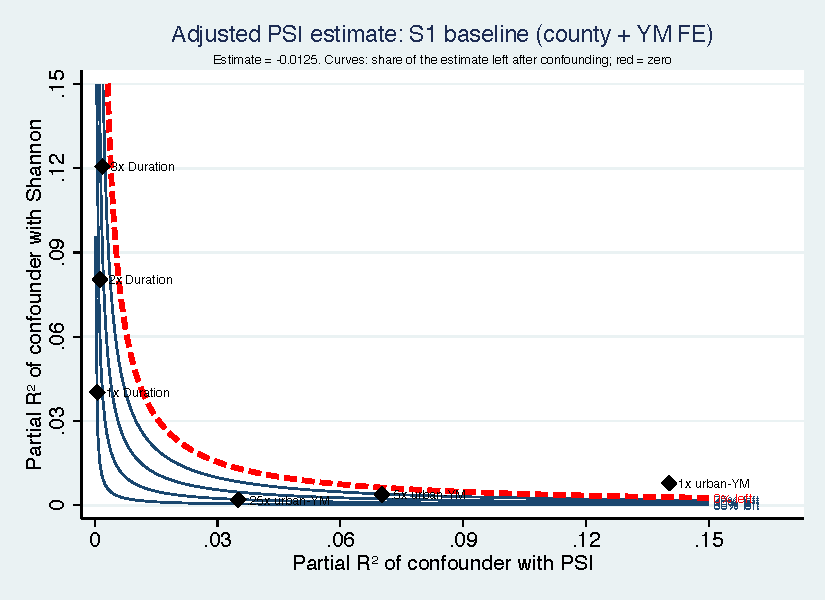
\includegraphics[width=0.78\linewidth]{fig/2_1_contour_estimate_S1.pdf}
\caption{Adjusted effect for hidden factors of different strengths (paper's model).}
\end{figure}
\begin{whybox}\small
\textbf{How to read Graph 1.}
\begin{itemize}[leftmargin=12pt]
\item \textbf{Bottom-left corner:} no hidden factor, so the effect is the paper's $-0.0125$.
\item \textbf{Blue curves:} how much of the effect is left (80\%, 60\%, \dots) as the hidden factor gets stronger.
\item \textbf{Red dashed curve:} the effect is \textbf{zero}. Beyond it, the effect flips to positive.
\item \textbf{``Duration'' diamonds:} a hidden factor 1, 2 or 3 times as strong as birdwatching effort, the strongest control in the paper. They sit high up but close to the left edge, because effort explains a lot about birds but almost nothing about policy.
\item \textbf{``urban-YM'' diamonds:} a hidden factor 0.25, 0.5 or 1 times as strong as the city-vs-countryside trend. They sit far to the right because this trend explains a lot about policy.
\end{itemize}
\textbf{Main message:} the red curve hugs the axes, so a weak hidden factor is enough. The ``1$\times$ urban-YM'' diamond lies \emph{beyond} the red curve, so a factor as strong as the city-vs-countryside trend would turn the effect positive ($+0.008$).
\end{whybox}

\subsection{Graph 2: when does the effect stop being reliable?}
\begin{figure}[H]\centering
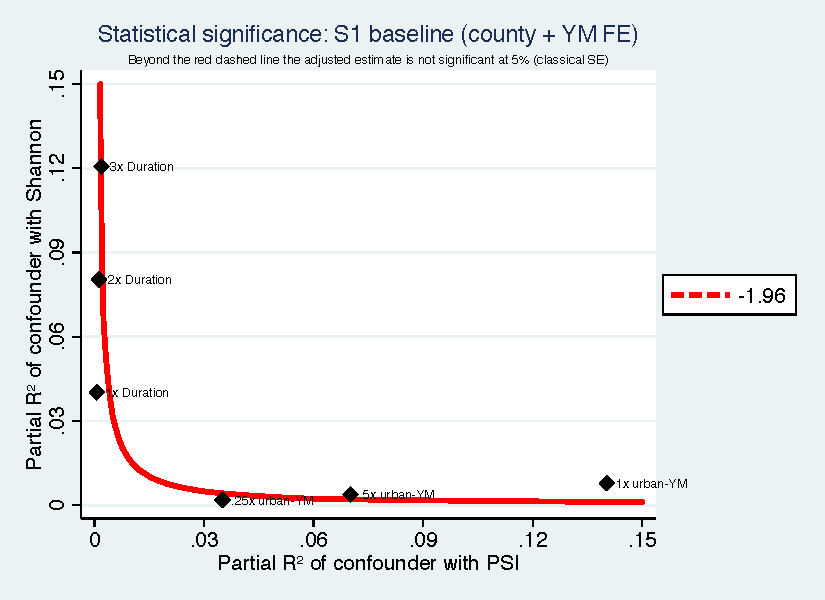
\includegraphics[width=0.78\linewidth]{fig/2_1_contour_tvalue_S1.pdf}
\caption{Where the result stops being statistically significant (paper's model).}
\end{figure}
\begin{whybox}\small
\textbf{How to read Graph 2.} Same axes. The red line now marks where the effect becomes \textbf{possibly chance} ($t=-1.96$). All three ``urban-YM'' diamonds are beyond it. For birdwatching effort, a factor \textbf{twice} as strong already makes the result borderline (clustered $t=-1.92$), and \textbf{three times} as strong makes it clearly not significant.
\end{whybox}

\begin{table}[H]\centering\small
\caption{The effect after allowing for a hidden factor like a known one}
\begin{tabular}{lccc}
\toprule
If the hidden factor were\dots & New effect & $t$ (clustered) & Still reliable?\\
\midrule
1$\times$ birdwatching effort & $-0.0096$ & $-2.69$ & Yes\\
2$\times$ birdwatching effort & $-0.0067$ & $-1.92$ & \textbf{No (just)}\\
3$\times$ birdwatching effort & $-0.0038$ & $-1.11$ & No\\
0.25$\times$ city-vs-countryside trend & $-0.0077$ & $-2.08$ & Borderline\\
\textbf{0.5$\times$ city-vs-countryside trend} & $\mathbf{-0.0027}$ & $-0.72$ & \textbf{No}\\
1$\times$ city-vs-countryside trend & $+0.0081$ & $+2.05$ & Sign flips\\
\bottomrule
\end{tabular}
\par\smallskip\footnotesize The other controls (temperature, wind, population, carbon, land cover) barely change the effect even at 3$\times$, because they hardly relate to solar policy.
\end{table}

\subsection{Graph 3: after adding the city-vs-countryside trend}
\begin{figure}[H]\centering
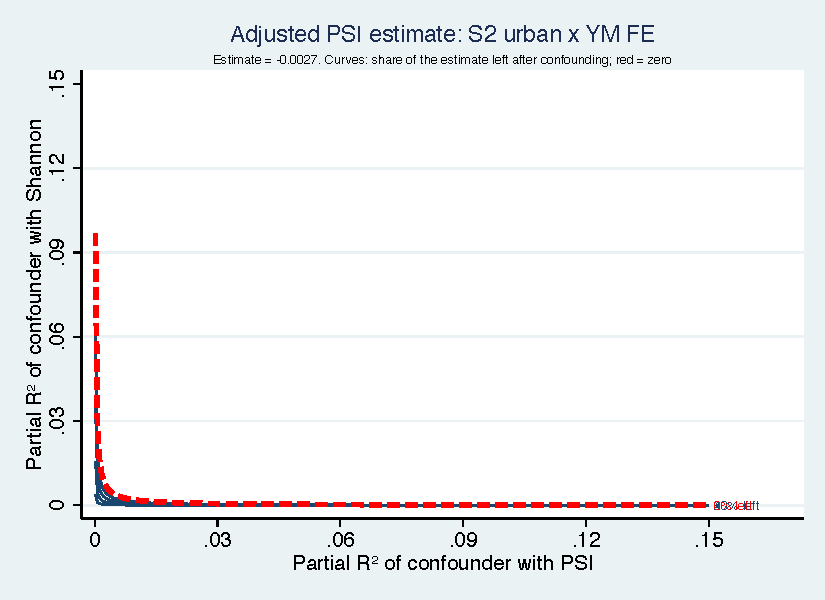
\includegraphics[width=0.7\linewidth]{fig/2_1_contour_estimate_S2.pdf}
\caption{Same graph after giving cities and countryside their own monthly trends.}
\end{figure}
\begin{whybox}\small
\textbf{How to read Graph 3.} The effect now starts at only $-0.0027$. The red ``zero'' curve is pressed flat against the axes, so \emph{almost any} hidden factor would remove it. There is basically nothing left to explain away.
\end{whybox}

%==========================================================================
\section{Task 3: Following counties before and after their first solar policy}

\subsection{The idea}
Counties started solar policy in different years (2015 to 2023). A newer group of methods handles this properly. For each county, we compare bird diversity \textbf{before and after its first solar policy} with counties that had not started yet (or never started). Older regressions can give wrong answers in this setting because they sometimes use already-treated counties as the comparison group.

\begin{itemize}
\item \textbf{Treatment:} the first year a county has any solar policy.
\item \textbf{Groups:} never treated 120; started in 2015: 299; 2016: 85; 2017: 75; 2018: 14; 2019: 68; 2020: 2; 2021: 91; 2022: 30; 2023: 155.
\item \textbf{Main sample:} only counties with real policy data. We also ran a ``paper-style'' version where missing-data cities count as ``never had policy''.
\end{itemize}

\subsection{How to read the event-study graphs}
\begin{whybox}\small
\begin{itemize}[leftmargin=12pt]
\item \textbf{x-axis:} years relative to the first solar policy. 0 is the first year; $-1$ is the year before (used as the reference, so it is set to 0).
\item \textbf{Dots:} the estimated difference in bird diversity in that year, compared with similar counties.
\item \textbf{Vertical lines:} 95\% confidence intervals. If a line crosses the dashed zero line, that year's effect could be chance.
\item \textbf{Left of the dotted line (before policy):} the dots should be near zero. If they are not, the two groups were already moving differently before the policy, and the comparison is less trustworthy.
\item \textbf{Right of the dotted line (after policy):} if solar policy harmed birds, these dots would \textbf{drop below zero}.
\end{itemize}
\end{whybox}

\subsection{Main sample: counties with real policy data}
\begin{figure}[H]\centering
\begin{subfigure}{0.49\linewidth}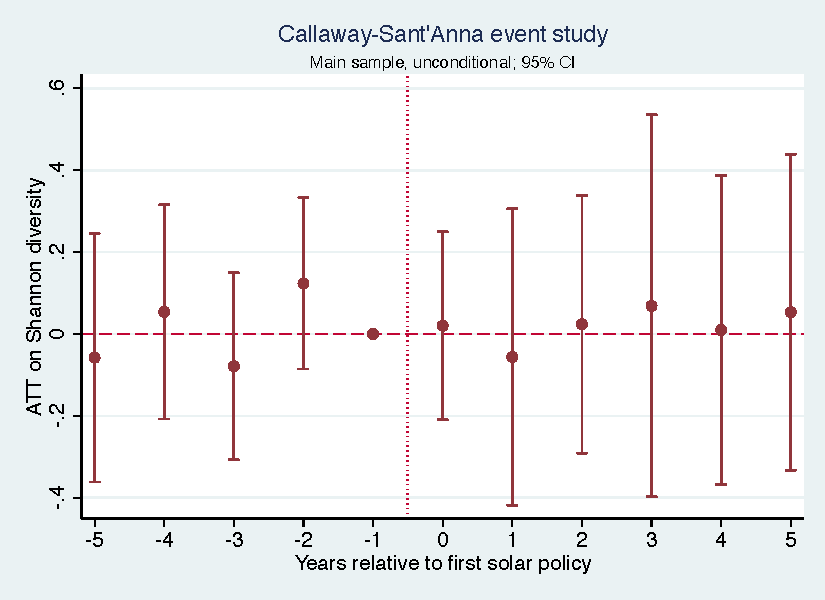
\includegraphics[width=\linewidth]{fig/3_3_event_study_cs_1.pdf}\caption{Callaway--Sant'Anna}\end{subfigure}
\begin{subfigure}{0.49\linewidth}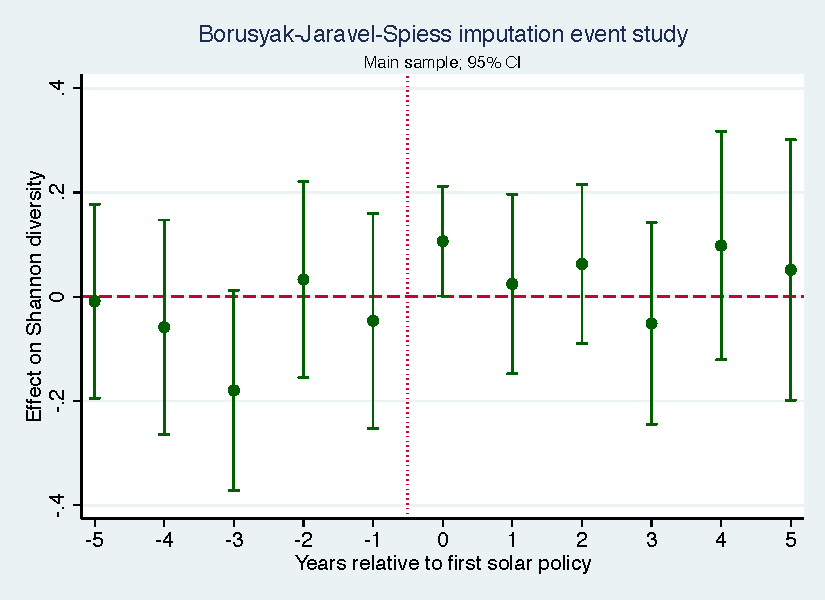
\includegraphics[width=\linewidth]{fig/3_4_event_study_bjs_1.pdf}\caption{Borusyak--Jaravel--Spiess}\end{subfigure}\\[4pt]
\begin{subfigure}{0.49\linewidth}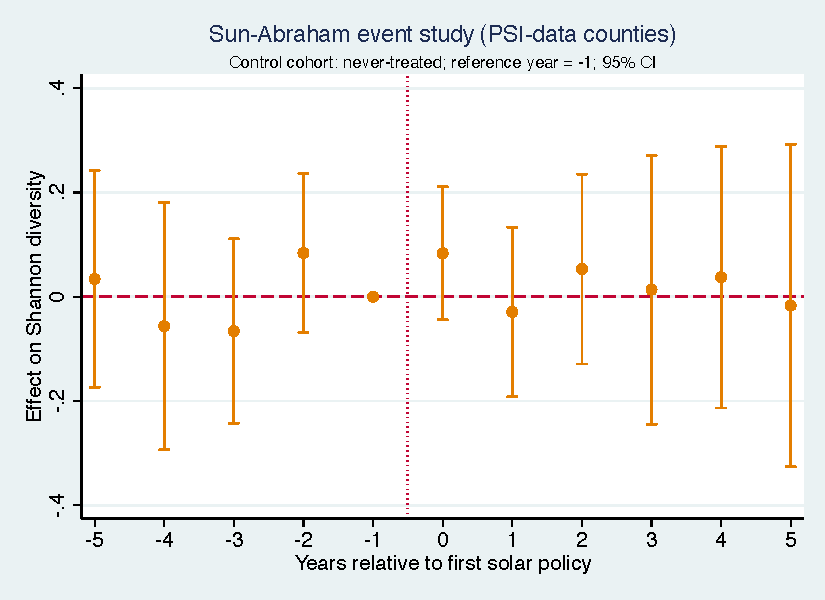
\includegraphics[width=\linewidth]{fig/3_5_event_study_sa.pdf}\caption{Sun--Abraham}\end{subfigure}
\begin{subfigure}{0.49\linewidth}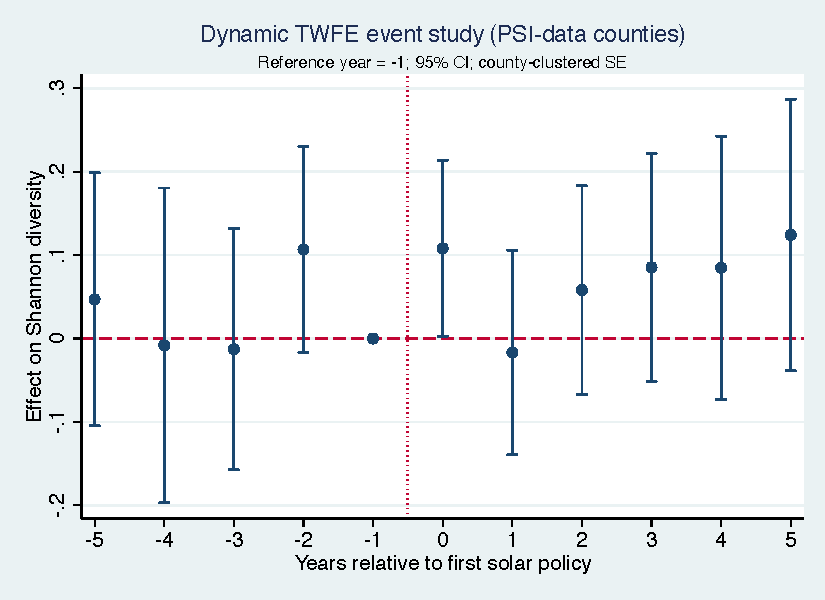
\includegraphics[width=\linewidth]{fig/3_2_event_study_twfe.pdf}\caption{Older regression event study (for comparison)}\end{subfigure}
\caption{Bird diversity before and after a county's first solar policy (main sample).}
\end{figure}
\begin{whybox}\small
\textbf{What these show.} In all four graphs, the dots after the policy (0 to 5) stay around zero or slightly \emph{above} it, and almost every line crosses zero. \textbf{There is no drop in bird diversity after solar policy starts.} The only years that look different from zero are year 0 in BJS and in the older regression (about $+0.11$), which are \emph{increases}, not declines. Before the policy, the dots wander around zero, with one dip at $-3$ in BJS.
\end{whybox}

\begin{table}[H]\centering\small
\caption{Average effect after the first solar policy}
\begin{tabular}{lccc}
\toprule
Method & Effect & Could it be chance? & Shows harm?\\
\midrule
Callaway--Sant'Anna & $+0.057$ (SE 0.143) & Yes & No\\
\quad same, comparing within city/countryside & $+0.057$ (SE 0.141) & Yes & No\\
Borusyak--Jaravel--Spiess & $+0.078$ (SE 0.069) & Yes & No\\
Sun--Abraham (years 0--5) & $+0.024$ (SE 0.089) & Yes & No\\
Older regression (static) & $+0.032$ (SE 0.041) & Yes & No\\
\bottomrule
\end{tabular}
\end{table}

\subsection{Paper-style sample: missing-data cities counted as ``never had policy''}
\begin{figure}[H]\centering
\begin{subfigure}{0.49\linewidth}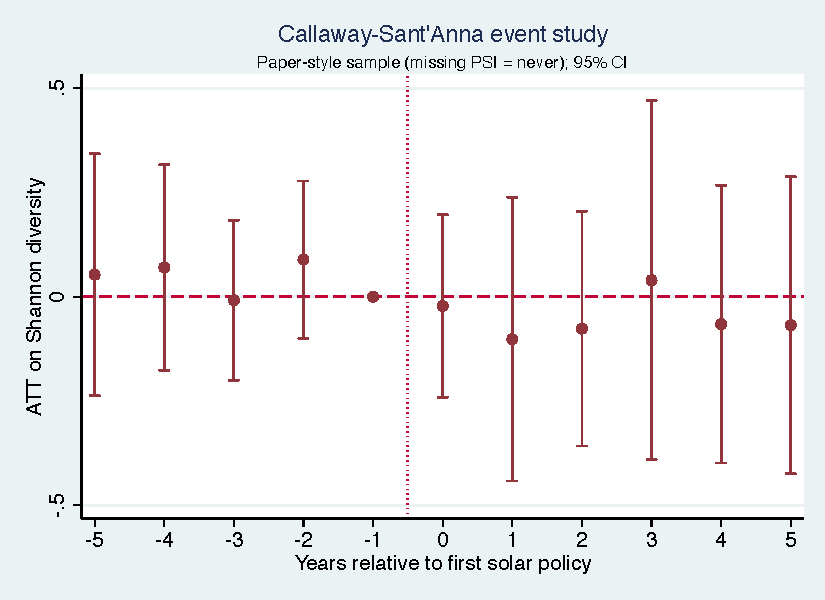
\includegraphics[width=\linewidth]{fig/3_3_event_study_cs_3.pdf}\caption{Callaway--Sant'Anna}\end{subfigure}
\begin{subfigure}{0.49\linewidth}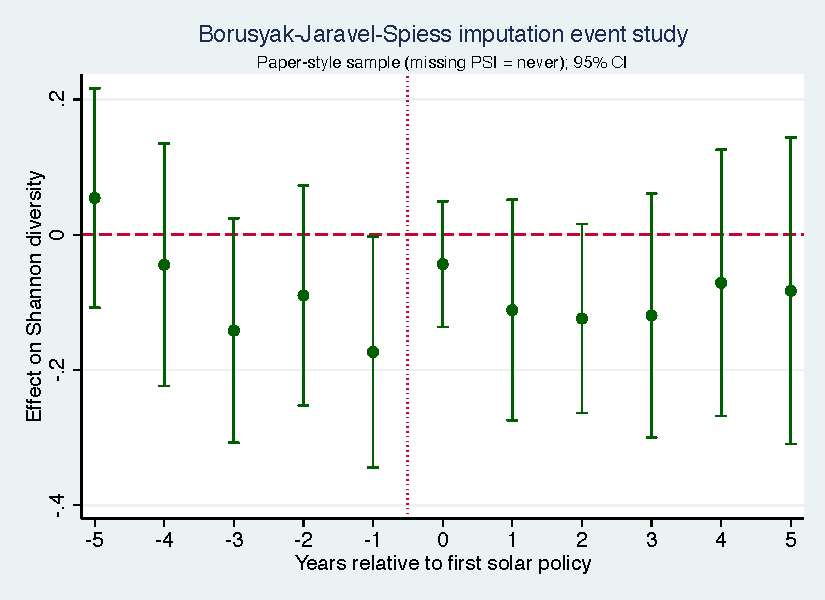
\includegraphics[width=\linewidth]{fig/3_4_event_study_bjs_2.pdf}\caption{Borusyak--Jaravel--Spiess}\end{subfigure}
\caption{The same analysis using the paper's choice for missing data.}
\end{figure}
\begin{whybox}\small
\textbf{What these show.} Once the missing-data cities are used as the comparison group, the dots after the policy turn \textbf{negative} (CS $-0.091$, BJS $-0.087$, both possibly chance). But look \emph{before} the policy in the BJS graph: the dots are already below zero, and at $-1$ the gap is $-0.173$, a clear difference. Bird diversity in these counties was \textbf{already falling relative to the cities before any solar policy}. So the negative ``effect'' is a difference that existed beforehand, not something caused by the policy. This is the same city-vs-countryside problem as in Task 1.
\end{whybox}

\paragraph{One honest caveat.} A formal test rejects ``no difference before the policy'' for Callaway--Sant'Anna ($p<0.001$), although the BJS test ($p=0.24$) and the older regression's test ($p=0.34$) do not. Some groups are also very small (only 2 counties started in 2020). So these designs are not perfect. But \textbf{none of them shows harm}.

%==========================================================================
\section{What we can and cannot say}

\begin{table}[H]\centering\small
\begin{tabularx}{\linewidth}{>{\raggedright\arraybackslash}p{3.4cm}>{\raggedright\arraybackslash}X>{\raggedright\arraybackslash}p{3.6cm}}
\toprule
Test & What we found & Supports harm?\\
\midrule
Fair comparison (Task 1) & Effect falls from $-0.0125$ to $-0.0027$, could be chance & No\\
Hidden factor (Task 2) & A factor explaining 1--2\% would remove it; city vs countryside is far bigger & No, result is shaky\\
Before vs after (Task 3) & All four methods: small, positive, could be chance & No\\
Backup methods (Task 1) & Instrument fails its key test; matching done wrong & No\\
\bottomrule
\end{tabularx}
\end{table}

\begin{summarybox}
\small
\textbf{What we can say:} ``When we compare similar places, test for hidden factors, or follow counties before and after their first solar policy, the negative effect either disappears or turns slightly positive and could be chance. So this study's data do not show that solar policy harms bird diversity. The negative result is most likely caused by comparing countryside counties with cities that have missing data.''\\[4pt]
\textbf{What we should NOT say:} ``Solar policy has no effect on birds'' or ``solar is good for birds.'' Our estimates are too uncertain to prove either. We can only say \textbf{this study does not prove harm}.
\end{summarybox}

\section*{Where to find everything}
\begin{tabularx}{\linewidth}{l>{\raggedright\arraybackslash}X}
Task 1 & \file{01\_Task1\_Replication/} (\file{1\_4} reproduction check, \file{1\_5} fair-comparison tests, \file{1\_6} instrument tests)\\
Task 2 & \file{02\_Task2\_Sensitivity/} (\file{2\_1\_sensitivity\_analysis.do}; graphs in \file{figures/})\\
Task 3 & \file{03\_Task3\_Staggered\_DiD/} (\file{3\_2} to \file{3\_5}; graphs in \file{figures/})\\
\end{tabularx}

\vspace{4pt}
\noindent{\small\textbf{Key readings:} Cinelli and Hazlett (2020), \textit{JRSS-B} 82(1): 39--67. Baker et al., ``Difference-in-differences designs: a practitioner's guide'', \textit{Journal of Economic Literature} (jel.20251650). Zhang et al.\ (2026), \textit{Science} 393, 831.}

\end{document}
